\section{The Predictive Performance measure \label{Chapter8:Predictive Performance}}

In the previous Sections, I have demonstrated that information flow measurements 
provide an index of how well each reflex and predictive pathway are used.
In this Section, I will combine the information flow measurements with the reflex entropy
to generate a single value which measures the learning performance.
This scalar value is called Predictive Performance.

\subsection{Introduction to closed loop measures}
In my research study, I formulated a novel closed loop information measure -
called predictive performance - which quantifies the learning
performance of a line following robot. The robot is a classical
Braitenberg vehicle\nomenclature{Braitenberg Robot}{An automated mobile robot with differential driving} (like the one described in Section \ref{Intro:Braitenberg}) 
which has 2 retinal inputs functioning as far
sensors and 2 small sensors acting as reflexes. The robot learns to
follow tracks of different complexity by developing a retinal field
using temporal sequence learning (ICO). I argue that measuring
only the retinal weights (input) or the angular motion (output)
provides a wrong estimate about the robot's adaptation to the track
curvature. Thus an objective measure of the robot's performance
-track deviation- is compared against the retinal field map and
against the predictive performance measure. Simulations show that a
robot with poor track performance has low retinal weights and a low
predictive performance. Whereas a robot with a good track
performance has high retinal weights and high predictive
performance. 
However a robot with a poor track performance could have high retinal weights ( I will explain why later),
but the predictive performance will be low thus giving an objective measure of the performance.
Therefore the predictive performance is a subjective
measure of adaptation which reflects the objective performance of
the robot. The measure can be extended to other types of adaptive
predictive controllers.

Information measures are usually defined for input/output systems
where they determine the quality of the transmission. Behaving agents,
however, act as closed loop systems (see Fig.\ref{PPmeasure:Figure1}) in which
there is no clearly defined difference between input and output because
the motor output influences the sensor input and so forth. What
matters most for the organism is to compensate for disturbances $P$
introduced by the environment into the perception action loop as in
Fig.\ref{PPmeasure:Figure1}(A). If there is no disturbance, the organism cannot
differentiate between themselves and the environment. Consequently,
the concept of information in these systems had to be revised
\citep{RadicalConstruct}.

\begin{figure}[!hbt]
	\begin{center}
		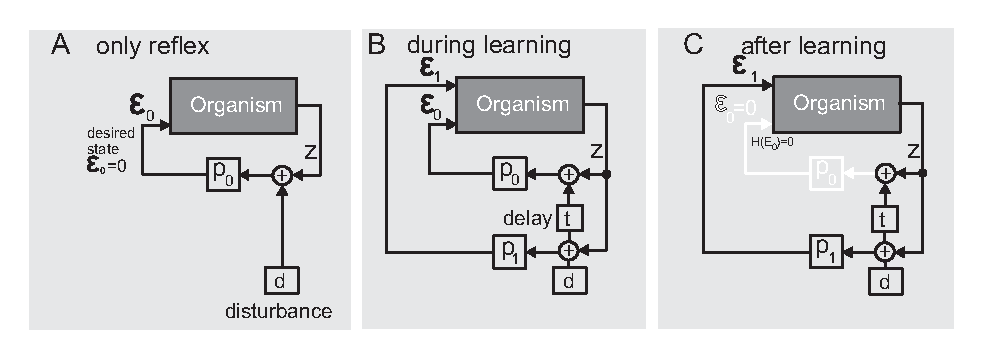
\includegraphics[width=0.9\textwidth]{figures/ppmeasure/1}
	\end{center}
	\caption[Information flow in the adaptive controller]{ 
	  {\bf A)} The organism is connected to the
          environment via the motor output $Z$ and the reflex sensory
          input $\epsilon_{0}$. The environment introduces a disturbance $d$
          via the transfer function $p_0$ which in turns change the
          reflex $\epsilon_{0}$. The organism wants to keep the reflex to 0, so
          its desired state is $\epsilon_{0}$.{\bf B)} An organism can learn to
          keep its desired state by using a predictive input $\epsilon_{1}$,
          providing that the disturbance $d$ acts on the reflex $\epsilon_{0}$
          with a delay of $t$. {\bf C)} After learning the organism
          should have reduced the reflex to 0 by using the predictive
          information $\epsilon_{1}$.  
	  \label{PPmeasure:Figure1}}
\end{figure}
 


The new information measure called 
\textsl{Predictive Performance} is motivated by the theoretical foundation of the 
Radical Constructivism as described by \citet{RadicalConstruct} stating that
everything that every organism has a model of the environment described
by his neural activity.
In essence the controller acts as a reactive system before learning and as an
open loop forward system after learning. In contrast to the
previous work my new measure is independent of the learning
rule and is not using its weights to compute the predictive
performance. Instead I have employed a purely information theoretical
approach.

I demonstrate my measure Predictive Performance in a simple
robotics task where a robot has to learn to follow a line which is laid
out with different curvatures so that different levels of difficulty
can be evaluated. Learning drives the development of receptive
fields in the robot similar to \citet{Kulvicius2007:RFrobot}. 
 
The Predictive Performance applied in this case, not only quantifies
the relative performance of the robot for the 3 different tracks but
also gives an index of the learning ability achieved by the robot
for every single track. Numerical simulations show that the robot
reduces the reflex information flow during learning and increases the
retinal information flow if learning was effective. More
specifically I show that an increase of Predictive Performance of
a pixel in the receptive field is not equivalent to a high weight
in the learning algorithm, which shows that one cannot rely on the
open loop property to predict the performance of the agent but
that instead it is necessary to use such a closed loop measure.

This rest of this section is divided as follows: setup of the robot,
learning architecture, task and performance, symbols and convention
used, application of the predictive requisite variety to a simple non
learning robot, then to a full learning robot and finally the discussion.


\begin{figure}[!hbt]
	\begin{center}
		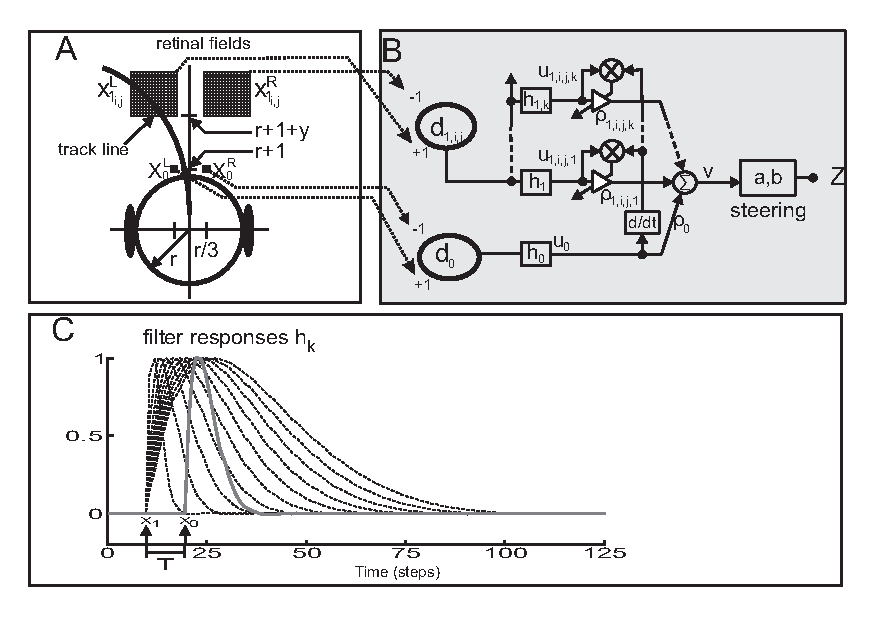
\includegraphics[width=0.9\textwidth]{figures/ppmeasure/2}
	\end{center}
	\caption[Retinal robot setup]{ Physical and neuronal setup of the receptive field
          (RF) development using the simple learning
          architecture. {\bf A)} Left and right retinal fields. The
          receptive filed positions are denoted by
          $x_{1_{i,j}}^{L,R}$, where $i=1 \ldots N_{rf}, j=1 \ldots
          N_{rf}$ are the indices of the RF pixels, and sensor field
          positions $x_0^{L,R}$. {\bf B)} The simple neuronal setup of
          the robot. Symbols $u$ 
          denote filtered input signals $x$, $\rho$ connection weights
          and $v$ the output of the neuron used for steering. $v$ is
          calculated by the method shown in C and its corresponding
          Eq.~\ref{NeuralOutput} given in Eq.~\ref{AngleComputation}
          and transforms $v$ to the motor output. $a$ is the
          acceleration gain and $b$ is the braking gain. 
          Schematic diagram of the learning system. Inputs $x$,
          resonator filters $h$, connection weights $\rho$, output
          $v$. The symbol $\otimes$ denotes a multiplication, $d/dt$ a
          temporal derivative. The amplifier symbol stands for a
          variable connection weight. Dashed lines indicate that input
          $x_1$ is fed into a filter-bank. {\bf C)} Resonator filters
          $h_0$ (solid line) for the input signal $x_0$ and $h_{1,k}$
          (dashed lines) for the $x_1$ given by parameters
          $f_{1,k}=2.5/k~Hz$, $k=1,\dots ,10$ for the filter-bank in
          the $x_1$ pathway. Frequency of the $x_0$ pathway was
          $f_0=1.25~Hz$. Damping parameter of all filters was
          $Q=0.6$. \label{PPmeasure:Figure2}}
	
\end{figure}



\subsection{Methods: experimental setup \label{Chapter8:RobotStructure}}

The agent's task is to follow a black track of constant width but
variable curvature in a 2 dimensional white arena.  The agent is
provided with a controller with a reflex steering behaviour which in
most of cases (except of very shallow turns) will not be sufficient to
steer the curve.  As a consequence the robot looses the track.
The learning goal is thus to learn predictive and smoother steering
reactions in order to stay on the track and to avoid the initial
reflex.

The reflex is generated by using two pixels close to the bottom of
the robot's visual field are are called $x_0^L$ and $x_0^R$ which
generate a difference signal $\epsilon_0$ which is used as the reflex
signal for steering and also drives learning of the receptive
fields.

The agent uses 2 predictive receptive fields $x_{1,i,j}^{L}$ and
$x_{1,i,j}^{R}$ for the left and right eye respectively. The receptive
fields have a size of $N_{rf} \times N_{rf}~px$ (Fig.~\ref{PPmeasure:Figure2}~A)
where each pixel within the receptive field represents an individual
input $x_{1,i,j}$. The left and right pixel intensities are then
combined into left and right difference signals pixel by pixel:
\begin{eqnarray}
\epsilon_0 & = & x_0^L(t) - x_1^R(t) \label{diffX0} \\
\epsilon_{1,i,j}(t) & = & x_{1,i,j}^{L}(t) - x_{1,i,j}^{R}(t) \label{diffX1}
\end{eqnarray}

All difference signals are then filtered by low pass filters
\begin{eqnarray}
u_0(t) & = & h_0(t) * \epsilon_0(t) \label{filterReflex} \\
u_{1,i,j,k}(t) & = & h_{1,k}(t) * \epsilon_{1,i,j}(t) \label{filterPred}
\end{eqnarray}
where $h_0(t)$ and $h_{1,k}(t)$ are 
low-pass filters which I define by its impulse
response:
\begin{equation}
	h(t)=\frac{1}{\beta}e^{\gamma t}\sin(\beta t),
\end{equation}
where, $\gamma=-\pi f/Q$ and $\beta={\sqrt{(2 \pi f)^2 - \gamma^2}}$,
with $f$ the frequency and $Q>0.5$ the damping. The index
$k$ in Eq.~\ref{filterPred} denotes a filter bank for the predictive
inputs so that every pixel of the receptive field is fed into $1\ldots K$
filters. This filter bank will be used for learning which is described
in the next section.

The filtered signals Eq.~\ref{filterReflex} and Eq.~\ref{filterPred}
are then fed into a summation unit where every signal
have a weight associated to it:
\begin{equation}
v = \rho_0 u_0 + \sum\limits_{i,j,k} \rho_{1,i,j,k} u_{1,i,j,k}
\label{NeuralOutput}
\end{equation}
where $v$ is is the steering angle which is calculated as the robot's
position in the cartesian bi-dimensional space ($S_x(t), S_y(t)$).

The robot has a constant speed of 1 Unit/s
\begin{eqnarray}
	s(t)& = & \Theta\left[speed-|v|\cdot b\right ]\\
	z(t)& = & z(t-1)-v(t) \cdot a \label{AngleComputation}
\end{eqnarray}
where $a$ is the acceleration gain 
$a=0.02$, $b$ is the breaking factor $b=0.005$ and $\Theta$
is the heaviside function.
$a$ controls the angular speed of the robot whereas $b$ simulates
breaking during turning.

\begin{eqnarray}
	S_x(t) & = & S_x(t-1)+s(t)\cdot\cos(z(t))\label{PositionComputationx}\\
	S_y(t) & = & S_y(t-1)+s(t)\cdot\sin(z(t))\label{PositionComputationy}
\end{eqnarray}
where $z(t)$ and $s(t)$ are computed in the previous equation
Eq.\ref{AngleComputation}.


\subsection{Methods: learning algorithm}

The temporal sequence learning rule was used again for learning \citep{Porr2006ICO}. 
The general scheme of such learning algorithm is presented in Fig.~\ref{PPmeasure:Figure2}~C. 

Weights change according to an input-input correlation (ICO) rule :
\begin{equation}
\dot\rho_{i,j,k} = \mu u_{i,j,k} \dot{u}_0,~~~j>0,
\end{equation}
which is a modification of the isotropic sequence order (ISO) learning rule \citep{Porr2003b}. 
The behaviour of this rule and its convergence properties are discussed in \citep{Porr2006ICO}. 
The indices $i$ and $j$ denote the different pixels and the index
$k$ is the filter number of the filter bank. 

The filter bank is needed to establish a temporal overlap of the
signals from the receptive field and the reflex
as demonstrated in
Fig.~\ref{PPmeasure:Figure2}C.
Remember that the
sensor fields $x_0^{L,R}$ are located at the bottom whereas sensor
fields $x_{1,i,j}^{L,R}$ are placed higher up from the reflex.

The time delay $T$ between the predictive receptive field $x_{1,i,j}$ and 
the reflex $x_0^{L,R}$ depends on the
speed of the robot and direction angle with respect to the
curvature. As shown in older studies of
\cite{Porr2003b,Porr2006ICO}, the number of filters $K$ is not critical and
here $K=10$ was used. The simulated robot has a speed of $1~Unit/s$
with filter coefficients $f_{k=1\ldots K}=0.1 k$, for the
filter-bank in the $x_{1,i,j,k}$ pathway. The frequency of the $u_0 = h_0 * x_0$ 
pathway was
$f_0=1.25~Hz$. Damping parameter of all filters was $Q=0.6$.



\subsection{Methods: symbols and conventions}

Before introducing the new measure Predictive Performance, it is necessary to
define the notation, symbols and information measures on which it is built. I am
first defining the used symbols, then introduce the necessary
information measures and finally, I will define my predictive performance.


\subsubsection{Symbols and conventions}

The symbols used in this section follows the convention:
\begin{itemize}
\item capital letters such as $X$ indicate a random discrete variable.
\item the symbols of the random variable are indicated by the set
  $X=\{x_1,x_2,...,x_S\}$ where $S$ is the number of symbols in this
set.
\item non capital letters such as $x$ indicate the corresponding
  discrete time series $x(k)$ from which I estimate the density
  $P(X)$ of the corresponding random variable $X$.
\item a time series is an ordered sequence of symbols
  $x(t)=\{x(0),x(1),...,x(t) \}$ for $t \geq 0$
\item the estimated entropy of a random discrete variable $X$ is
  identified by $H(X)$ and is measured in bits.
\end{itemize}
I then identify my controller with the following variables and
measures:
\begin{itemize}
 \item $E_{0}$: random variable for reflex input
 \item $E_{1,i,j}$: random variable for predictive input located at the retinal coordinate $i,j$
 \item $Z$: random variable for motor output
 \item $H( E_{0} ),H(E_{1}),H(Z)$: entropy of the random variables $E_0,E_1,Z$
 \item $I(X,Y)$= mutual information between variable $X$ and variable $Y$
 \item $MI^n(X,Y,\tau)$= mutual information of order $n$ between $X$ and 
	the delayed version of $Y$ by factor $\tau$ (see Appendix \ref{sec:MutualInfo} for more details)
 \item $MI(X,Y)=MI(X,Y,\tau=1)$ 
\end{itemize}

In the following subsections I am going to describe the different information measures
 which can be applied to the robot.
I show that these measures by themselves are not a good measure for the performance of 
the agent but combined will provide a measure which reflects the performance of the 
agent in a normalised way.
Initially I introduce the information measures, then I apply it in the closed loop
 and finally I combine to form the Predictive Performance.

\subsubsection{Input reflex entropy}
The entropy $H(E_0)$ is the uncertainty of the reflex input or the
average description necessary to encode the reflex input $D_{0}$. Before
I am going to look at the actual values I need to recall that
the reflex input is part of the reflex loop (see Fig.~\ref{PPmeasure:Figure1})
via the differences of $x_0^L-x_0^R$, 
$v_0$, $z$, the environment $p$ and back to $\epsilon_0$. This
loop is disturbed by the perturbation $d$ which is then eliminated
by the loop. Remember that $\epsilon_0$ is essentially an error signal which has to be
kept close to zero which is only the case for Eq.~\ref{d0time2}.
However, because it is a reflex loop the feedback
loop always reacts too late so that the input $\epsilon_0$ can never
reach a constant value. Thus, the entropy at $\epsilon_0$ reflects the
entropy originating from $d$. In my
setup the reflex has an alphabet of 3 symbols $E_0=\{-1,0,1\}$ to
encode the line position on the left, right or center. The condition
$H(E_0)=0$ of null entropy, indicates that the closed loop controller
has achieved perfect regulation, however there are 3 possible
conditions with equal null input entropy:
\begin{eqnarray}
\epsilon_{0}(t) & = \{1 ,1, 1, 1\} & \rightarrow H(E_0)=0 \label{d0time1} \\
\epsilon_{0}(t) & = \{0, 0, 0, 0\} & \rightarrow H(E_0)=0 \label{d0time2} \\
\epsilon_{0}(t) & = \{-1, -1, -1, -1\} & \rightarrow H(E_0)=0 \label{d0time3}
\end{eqnarray}
I can exclude condition Eq.~\ref{d0time1} and Eq.~\ref{d0time3} because
they only arise when the feedback loop has failed totally.
In order to have a successful learning, it is required at least a working feedback 
loop \citep{RadicalConstruct} as a starting point.
A perfect organism would have an input sequence identical to Eq.~\ref{d0time2},
 however due to the causal nature of the sensory-motor loop there will be always a 
delay between the reaction and the disturbance as in  Eq.~\ref{d0time4} and Eq.~\ref{d0time5}.
Thus there is never  zero entropy at $\epsilon_0$ as long as the reflex keeps the robot on track:
\begin{eqnarray}
\epsilon_0(t)=\{-1, 0, 1, 0, -1, 1\} &\rightarrow  H(E_0)=1.6\label{d0time4}\\
\epsilon_0(t)=\{-1, -1, 0, 0 ,1, 1\} &\rightarrow  H(E_0)=1.6\label{d0time5}
\end{eqnarray}
the entropy reaches a maximum of 1.6 bits which means that the input
has a uniform distribution and thus is not constant in time. The
input entropy does not tell us anything about the effort that the
controller is doing to keep its desired goal, because it might be that
the robot is not moving at all or that the environment is very
simple (e.g. straight line). For that reason I need to define
now truly closed loop measures.


\subsubsection{Retinal predictive entropy}
Remember that the goal of the learning algorithm is to make
the reflex pathway redundant. In order to achieve this
it aims to predict the trigger of the reflex via the reflex
input (see Eq.~\ref{diffX0})
with the predictive inputs of originating from the
difference of the receptive fields (see Eq.~\ref{diffX1}).

I define $H(E_{1,i,j})$ as the uncertainty of the predictor
inputs at the retinal position $(i,j)$, whereas 
\begin{equation}
H(E_{1})=\frac{1}{N_{rf}^2}\cdot \sum\limits_{i,j=1}^{N_{rf}} H(E_{1,i,j})
\end{equation}
is the average entropy of the retinal differential input.

\subsubsection{Mutual information}
\label{sec:MutualInfo}
The previous sections described only input measures but I also need additional
 measures calculated between the output and the input of the agent to measure
the information flow in the closed loop.
The mutual information takes into account the performance of the controller
by measuring how the controller reacts to the error signals at the
reflex and predictive inputs:
\begin{enumerate}
\item $MI(Z,E_0,\tau,n)$: mutual information of the reflex loop
\item $MI(Z,E_{1,i,j},\tau,n)$: mutual information of the predictive loop for
  the single input $E_{1,i,j}$
\item $MI(Z,E_1,\tau,n)$: average mutual information of the predictive loop
  which is computed as:
  \begin{equation}
    MI(Z,E_{1})=\frac{1}{N_{rf}^2}\cdot \sum\limits_{i,j=1}^{i,j=N_{rf}} I(Z,E_{1,i,j},\tau,n)
  \end{equation}
\end{enumerate}
where the parameter $\tau$ is the temporal difference between the motor output $z$ 
and the sensory input $\epsilon_0,d_{1,i,j}$ and $n$ is the sensory integration window.
For instance when computing $MI(Z,E_0,\tau,n)$, I am considering as the 
random variable $Z$ the motor output $z(k)$ and as random variable $E_0$ the
sensory input sequence $d_{0}(k+\tau),d_{0}(k+\tau+1),...,d_{0}(k+\tau+n-1)$. 
When $\tau$ and $n$ are omitted that indicates that the mutual information has been maximised 
over the 2 parameters:
\begin{equation}
MI(Z,E_{0/1,i,j})=\max_{\tau,n} MI(Z,E_{0/1,i,j},\tau,n)
\end{equation}

The mutual information $MI(Z,E_0),MI(Z,E_{1,i,j})$ is a measure of the 
\textit{controllability} of the agent. To demonstrate this
I show the two extreme cases:
\begin{itemize}
\item if $MI(Z,E_0)=0$ then $Z$ and $E_0$ are independent.  It means
  that there is no correlation between the actions and the inputs of
  the robot.  Imposing a motor value does not give a desired input.
  For example the series:
 \begin{eqnarray}
z(t) & = &\{1, 2, 3, 4 ,5 ,6\}\\
\epsilon_{0}(t)& =&\{-1 ,0 ,-1, 1, -1 ,0, 1\}
\end{eqnarray}
have null mutual information $MI(Z,E_0,\tau=1)=0$ bits.
\item if $MI(Z,E_0)=max(H(Z),H(E_0))$ then $Z$ and $E_0$ are perfectly
  dependent.  It means that this time when the robot imposes a motor
  action it will have a better chance of reading a desired input.  For
  example if $MI(Z,E_0)=1.6$ bits, then the robot can choose a motor
  action and read a desired input in an average run.  But if the robot
  looses 0.6 bit and goes to $MI(Z,E_0)=1.0$ then in the average run 1
  particular motor action will yield 2 equiprobable inputs at $E_0$ and
  thus the robot has less control over its environment.
\end{itemize}
An equivalent description of the mutual information can be done with
the conditioned entropy:
\begin{eqnarray}
MI(Z,E_0) & = & H(E_0)-H(E_0|Z)\\
MI(Z,E_{1,i,j}) & = & H(E_{1,i,j})-H(E_{1,i,j}|Z)
\end{eqnarray}
Here $H(E_0|Z)$ and $H(E_{1,i,j}|Z)$ are the conditional entropies. 
Since $H(E_0)\geq H(E_0|Z)$,
this characterization is consistent with the non negativity property
of entropy. If entropy $H(E_0)$ is regarded as a measure of
uncertainty about a random variable, then $H(E_0|Z)$ is a measure of
how much the motor output $Z$ has no influence over the input $E_0$.
This is the amount of uncertainty remaining about $E_0$ after $Z$ is
chosen, and thus the right side of the first of these equalities can
be read as the amount of uncertainty in $E_0$, minus the amount of
uncertainty in $E_0$ which remains after $Z$ is chosen, which is
equivalent to the amount of uncertainty in $E_0$ which is removed by
imposing $Z$.  In a broader sense the mutual information $MI(Z,E_0)$
measures the quantity of information that the robot is able to recover
from its inputs given its outputs.  In control theory I can think
about the $MI(Z,E_0)$ as a measure of the controllability: if it is 
maximum it means the robot can reach any desired input by a determined
action, if not the robot cannot reach certain desired states with
absolute certainty.

However, the mutual information via the reflex or the predictive
pathway itself is not sufficient as a performance measure. Remember
that I would like to measure the success of learning, especially if it
is using the predictive
pathway via $\epsilon_{1,i,j}$ to eliminate the pathway via $\epsilon_0$.
In other words I need to verify if the mutual information is
transferred from the reflex to the predictive pathway \textsl{and}
that the error of the reflex has been reduced to $\epsilon_0=0$ after learning. 
I combine these requirements in one measure called 
``predictive performance'' which I am describing in the
next section.


\subsection{Methods: Predictive Performance measure}
The predictive performance measure is computed by considering the
information measures introduced before. The subscript $t=0$ and $t=\infty$ indicate
respectively the measure computed before learning and after learning after the weights 
have been stabilised.
Table \ref{table:PPmeausure:Values} contains the four values that are relevant
to the agent's performance:

\begin{table}[htbp]
\caption[Information values for the \textbf{PP} computation]
{Information measures used for the computation of Predictive Performance. \label{table:PPmeausure:Values}}
\begin{center}
  \begin{tabular}{| l | l | l | l |}
    \hline
		    & $H(E_0)$ & $MI(Z,E_{1,i,j})$ & $MI(Z,E_0)$\\ 
    \hline
    before learning & $H(E_0)_{t=0}$ & $MI(Z,E_{1,i,j})_{t=0}$ & $MI(Z,E_0)_{t=0}$ \\ 
    \hline
    after learning &  $H(E_0)_{t=\infty}$& $MI(Z,E_{1,i,j})_{t=\infty}$ & $MI(Z,E_0)_{t=\infty}$ \\ 
    \hline
  \end{tabular}
\end{center}
\end{table}

The predictive performance is then computed as:
\begin{equation}
PP_{i,j}= \frac{H(E_0)_{t=0}-H(E_0)_{t=\infty}}{H(E_0)_{t=0}}\cdot 
\frac{MI(Z,E_{1,i,j})_{t=\infty}}{MI(Z,E_0)_{t=0}}
\label{eq:PPmono}
\end{equation}
The two factors of this equation need to be discussed now:
\begin{itemize}
\item The first factor of Eq.~\ref{eq:PPmono} provides a measure
  reflecting the reduction of entropy of the error signal $E_{0}$
  which drives the reflex. Remember that the goal of learning is to
  avoid the reflex which in an ideal case will lead to no trigger of
  the reflex or $\epsilon_0=0$. In a realistic scenario the reflex entropy
  will decrease but the never reach zero because the agent might do
  mistakes from time to time.  In general the entropy should be lower
  after learning than before: $H(E_0)_{t=0}\geq H(E_0)_{t=\infty}$.
  Thus, the first factor in Eq.~\ref{eq:PPmono} will be one for
  perfect avoidance of the reflex and zero for no change in the reflex
  entropy.
\item The second factor makes sure that the agent controls its own
  actions before ($MI(Z,E_0)_{t=0}$) and after
  ($MI(Z,E_{1,i,j})_{t=\infty}$) learning. This factor makes sure that
  before and after learning the agent is able to generate actions
  which control its own inputs. Remember that before learning this is
  done via the reflex input and that this is my starting point. After
  learning the agent should be in control of its own actions via the
  predictive inputs.  Ideally, these two mutual information values
  should be similar which means that control before and after is
  guaranteed. Or in other words, the controllability should be
  transferred from the reflex ($MI(Z,E_0)_{t=0}$) to the predictor
  ($MI(Z,E_{1,i,j})_{t=\infty}$).
\end{itemize}

An example of a perfect learner can be an agent with the following values:

\begin{center}
  \begin{tabular}{| l | c | c | c |}
    \hline
		& $MI(Z,E_0)$ & $MI(Z,E_{1,i,j})$ & $H(E_{0})$\\ \hline
    before learning & \textbf{2.5 bits} & 1.5 bits & \textbf{3 bits} \\ \hline
    after learning & 0 & \textbf{2.5 bits } & \textbf{0 bit}\\ \hline
  \end{tabular}
\end{center}
which results in a Predictive Performance of $PP=1$ (see Eq.~\ref{eq:PPmono}).
The important values here are in bold. The mutual information is completely transferred
from the reflex pathway to the predictive pathway and the error in $\epsilon_0$ is reduced 
to zero bits. In fact a necessary but not sufficient condition for learning is that 
$MI(Z,E_0)_{t=0} \cong MI(Z,E_{1,i,j})_{t=\infty}$ because the predictor should be able to
provide information that has to be learned or exploited by the controller.
The following section describes behavioural experiments conducted to demonstrate 
the predictive performance.

\subsection{Results: behavioural experiments}

\subsubsection{Task}
The task of the robot is to follow a track.
I designed tracks of increasing difficulty.
There are three simple tracks (see Fig.\ref{PPmeasure:Maps}(A)) with an increasing curvature ratio and a complicate
track (see Fig.\ref{PPmeasure:Maps}(B)) with left and right turns of different curvatures.
The retinal field that will be learned will have different structure for every track and the robot
will show a different level of performance.
\begin{figure}[!hbt]
	\begin{center}
		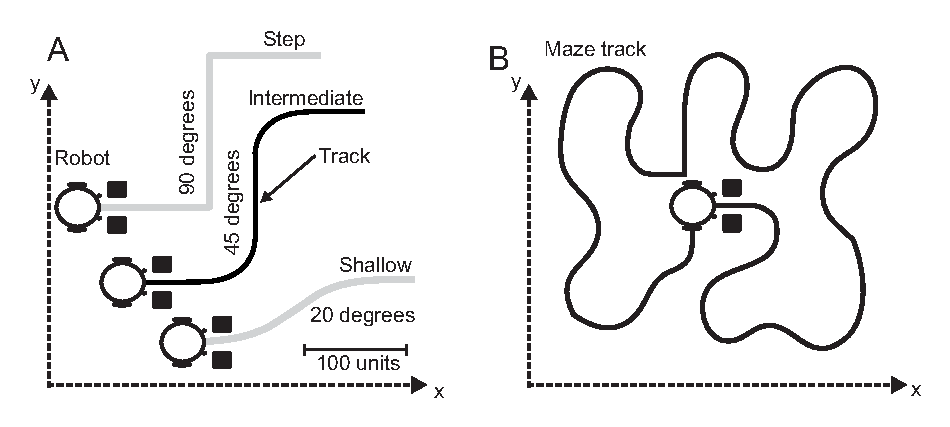
\includegraphics[width=0.9\textwidth]{figures/ppmeasure/3}
	\end{center}
	\caption[Track shape of increasing curvature]{
	{\bf A)} Three tracks of increasing difficulty: shallow, intermediate and step. 
	The Cartesian coordinate system has origin in the bottom left corner. 
	{\bf B)} A maze track with different curvatures, the robot starts in the middle.
	\label{PPmeasure:Maps}} 

\end{figure}

\subsubsection{Behavioural performance}
In order to assess the Predictive Performance, it is necessary to introduce an objective 
or behavioural performance. 
Learning is successful when the robot is not triggering the reflex any more, thus
minimising its distance from the track.
Thus the deviation from the track is simply defined as the
average deviation of the robot's position (defined by the mass centre
of the robot) from the track.  It is obtained from the robot's driving
trajectory and is calculated by the Euclidean distance:
\begin{equation}
\psi=\frac{1}{N_{sim}} \sum_{t=0}^{N_{sim}-1} \sqrt{(S_x(t)-x_t(t))^2+(S_y(t)-y_t(t))^2} \,\, units,
\label{deviation}
\end{equation}
where $S_x(t)$ and $S_y(t)$ are the coordinates of the robot's
position at time moment $t$, $x_t(t)$ and $y_t(t)$ are the coordinates
of the track point from which the distance to the robot's position is
minimal, and $t=0\ldots N_{sim}-1$ denote the driving duration and is
measured in simulation steps.  This measure $\psi$ will be used as an
objective measure of the robot's performance for each track type.


\subsubsection{A simple non-learning robot}
Before applying the Predictive Performance to a complex retinal based robot, it is
better to measure it on a simplified robot with few parameters and an intuitive behaviour.
The simplified robot is described in Fig.\ref{PPmeasure:Figure4} and to its parameters $k_1,k_2$,
it is possible to show how the predictive performance works when the robot
switches between the reflex pathway $\epsilon_0$ to the predictive pathway $\epsilon_{1,i,j}$ by
manually setting the gain of the reflex and predictor. The reflex
$x_0$ here is a digital $b/w$ line sensor and the predictor $x_{1,i,j}$ is a
$b/w$ retina of 4x4 pixels. The difference between the left and right
reflex $\epsilon_{0}$ is fed into a band pass filter to produce $u_{0}$. The
difference between the left and right retina $x_{1,i,j}$ is fed into 16
band pass filters to produce $u_{1,i,j}$. The distance between the
reflex and the predictor is $y$ and will assume the following values ($y=\{6,12,24\}$ units) 
to do a comparative analysis of the performance.\\

\begin{figure}[!hbt]
	\begin{center}
		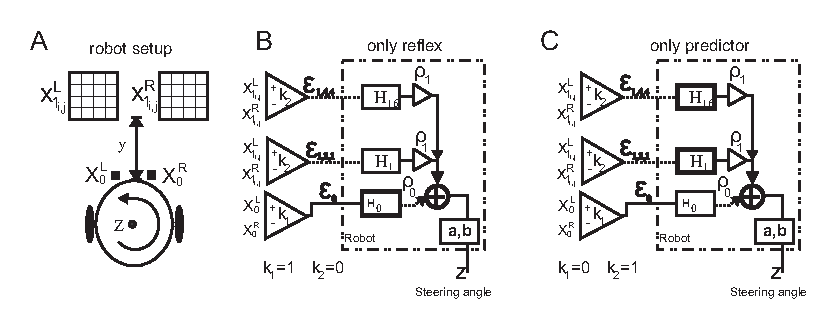
\includegraphics[width=0.9\textwidth]{figures/ppmeasure/4}
	\end{center}
	\caption[Simple retinal robot]{
	{\bf A)} A simple non learning robot with a 4x4 retinal field. 
	{\bf B)} In this configuration the robot uses only its reflex $\epsilon_0$ and ignores -while still experiencing- the predictor $\epsilon_{1,i,j}$. 
	{\bf C)} In this configuration the robot uses only its predictor $\epsilon_{1,i,j}$ and ignores -while still experiencing- the reflex $\epsilon_0$. 	
	\label{PPmeasure:Figure4}} 
\end{figure}

The neuronal output is computed as the synaptic input summation of the reflex and predictor:
\begin{equation}
  \begin{array}{ll}
	v(t)=k_1\cdot u_{0}+k_2 \sum\limits_{i,j}^{i,j=4} u_{1}\\ 
        \mu=0
  \end{array}
\label{MotorSimple}
\end{equation}
Where the parameters $k_1,k_2$ can be set to only test the reflex pathway when
$k_2=0$ and test the predictor pathway when $k_1=0$.
The robot is not learning anything because the learning speed is set to
zero -$\mu=0$- thus the weights are steady. The parameters $k_1,k_2,a,b,\rho_{1,i,j}$ are 
tuned manually so that the robot is able to complete the track.
The predictive information flow here is a simple average over the individual retina channels
because these channels have no specific meaning as they have been chosen manually.
The predictive information flow becomes:
 \begin{equation}
 MI(Z,E_1)=\frac{1}{16} \sum\limits_{i,j=1}^{i,j=4} MI(Z,E_{1,i,j})
 \end{equation}
indicating that Eq.\ref{eq:PPmono} for the PP is essentially reduced to a single pixel 
for the reflex and a single pixel for the predictor. 

Table \ref{table:PPmeausure:TableSimplePP} contains the computed parameters for 
the PP measure in the maze track scenario.
The first column shows the different distances $y$ between the predictor and the reflexes
in pixels which is used here to vary the level of difficulty for learning.
I am going to argue that both fractions in Eq.\ref{eq:PPmono} are needed to combine
the measures which include mutual information with the measure of the reflex entropy.


\begin{table}[htbp]
\addtolength{\tabcolsep}{-2pt}
\caption[Table with entropy values for simple robot]{Table measuring the predictive performance for different distances $y$ of the predictor as seen in Fig.\ref{PPmeasure:Figure4}(C). \label{table:PPmeausure:TableSimplePP}}
\begin{small}
\begin{center}
  \begin{tabular}{|l|c|c|c|c|c|c|c|c|}
    \hline
    $y$ & $\underbrace{MI(Z,E_0)}_{t=0}$ & $\underbrace{MI(Z,E_1)}_{t=0}$ & $\underbrace{MI(Z,E_0)}_{t=\infty}$& $\underbrace{MI(Z,E_1)}_{t=\infty}$ & $\underbrace{H(E_{0})}_{t=0}$ & $\underbrace{H(E_{0})}_{t=\infty}$ & $PP$ \\ \hline
     6 &4.16 bits&3.99 bits&0& 3.7 bits& 0.137551&0&0.89\\ \hline
     10 &4.16 bits&4.12 bits&0& 3.91 bits& 0.137551&0&0.939\\ \hline
     12 &4.16 bits&4.17 bits&0.0453& 3.91 bits& 0.137551&0.00536&0.902\\ \hline
  \end{tabular}
\end{center}
\end{small}
\end{table}

First of all the reflex input entropy $H(E_{0})$ is the standard measure
to evaluate the performance of a closed loop controller: the entropy is zero when
the desired state is achieved ideally after learning.
The sixth and seventh column of Table \ref{table:PPmeausure:TableSimplePP} contain
the input entropies of the reflex before $t=0$ and after $t=\infty$ learning.
When the distance is $y=6,10$ the reflex pathway is totally removed $H(E_{0})_{t=\infty}=0$,
whereas for the distance $y=12$ there is a remaining error of $H(E_{0})_{t=\infty}=0.00536$,
indicating that in very few occasions the robot sill needs to use its reflex even when
the predictive pathway is performing most of the steering reaction.
This obviously contributes to a lower Predictive Performance in the last row of the table.
Nevertheless, a zero input entropy at $\epsilon_0$ does not mean that learning has been
successful. For example, the robot could have just driven into an easier section of a track
like a straight line where the absence of steering does not trigger any reflex.
This issue can now be solved by considering the mutual information between output and inputs
(see columns 2-5 in Table \ref{table:PPmeausure:TableSimplePP}).
The first column shows the mutual information of the reflex pathway $MI(Z,E_0)_{t=0}$
before learning which is identical for all cases.
The next column shows the mutual information of the predictive pathway $MI(Z,E_1)_{t=0}$
before learning that provides whether or not learning is possible.
A non-zero value indicates that the predictor is highly correlated with the output z
and therefore learning is possible.
The next two columns contains the mutual information for the reflex and 
predictive pathway after learning: a robot with an uncorrelated behaviour will generate
very low values for mutual informations.
An agent which has learned to use the predictive pathway will generate instead
high values for the mutual informations.

It is impossible to use only the mutual information of the reflex loop after learning
to determinate the performance because, for example when the distance is $y=6,10$
$MI(Z,E_0)_{t=\infty}=0$. This condition would indicate a total loss of control
in the robot but the interpretation is ambiguous because the reflex entropy $H(E_0)\simeq 0$
is almost null because $\epsilon_0$ is converging to zero. This basically means that 
the reflex pathway after learning $MI(Z,E_0)_{t=0} \simeq 0$ becomes unused.

However there is an important property that has to be observed: when the agent
transfer its control from the reflex pathway to the predictive pathway the mutual information
has to be transferred as well from the reflex pathway $MI(Z,E_0)_{t=0}$ to the
predictive pathway $MI(Z,E_0)_{t=\infty}$.
Table \ref{table:PPmeausure:TableSimplePP} clearly show how the initial information flow
of the reflex pathway which is about 4.16 bits is transferred to the information flow
of the predictor pathway almost intact (just a little less than 4 bits) for the cases
$y=10,12$. For the short configuration $y=6$ the reduction was from 4.16 to 3.7 bits
but this is due to the manual setup of the weights.

This is the reason why the predictive performance uses both the input entropy 
$H(E_{0})$ and the mutual information $MI(Z,E_0)_{t=0}$ before learning and
after learning $MI(Z,E_0)_{t=\infty}$.

The last column of Table \ref{table:PPmeausure:TableSimplePP} contains the predictive
performance computed for each parameter setting of the $y$ distance.
The maximum value is achieved when $y=10$ because there is a good information transfer
from the reflex to the predictor pathway $4.16 \rightarrow 3.91 $ bits and a null
input entropy after learning $H(E_1)=0$.
For $y=12$ the performance is lower because the input entropy after learning
$H(E_1)=0.00536$ the input entropy is bigger then 0.
The worse performance is for $y=6$ because of the lower information transfer
$4.16 \rightarrow 3.7 $ but with null input entropy after learning $H(E_1)=0$.
This shows that minimizing the reflex entropy it not sufficient to generate a
controllable robot.

The best performance $PP=0.939$ is achieved when the predictor-reflex distance is 
at $y=10$, but how does it relates to the real objective performance of the robot?
Table \ref{table:PPmeausure:TableSimpleTrack} provides the answer by computing the
track deviation when the robot is following the track.
For instance when the PP is maximum for $y=10$ the track deviation $\Psi\simeq4.038$
is minimum, whereas for the worse performance when $y=6$ the PP is minimum and 
the track deviation is maximum $\Psi\simeq4.95$.
This relationship between PP and $\Psi$ indicates that the predictive performance
is well correlated with the objective track performance of the robot.
The first row in Table \ref{table:PPmeausure:TableSimpleTrack} also measures
the track deviation when the robot is only using the reflex $\Psi\simeq 1.93$ and 
shows that after the robot switch to the predictive pathway the track deviation 
is bigger rather then smaller as one would expect for a learning robot.
Essentially a purely reflex 
based robot has the best performance $\Psi \simeq 1.93$ compared to the only predictor based case. 
This is because I have chosen the gain of the predictor field to an arbitrary gain
by ``hand'' that produces over steerings even though the robot is always on track.
Because the robot's retinal weights are manually set, it was not possible to 
achieve a better performance but for an autonomous learning robots 
learning must provide a better track deviation.

\begin{table}[htbp]
\caption[Track deviation values for simple robot]{Table measuring the track deviation $\Psi$ for the simple robot 
as seen in Fig.\ref{PPmeasure:Figure4}(B),(C) on the maze track. \label{table:PPmeausure:TableSimpleTrack}}
\begin{center}
  \begin{tabular}{| l | c | c |}
    \hline
     Mode & $\Psi$ \\ \hline
     only reflex & 1.936951 \\ \hline
     only predictor at $y=6$  & 4.959343\\ \hline
     only predictor at $y=10$ & 4.038652\\ \hline
     only predictor at $y=12$ & 4.119643\\ \hline
  \end{tabular}
\end{center}
\end{table}

The adaptive receptive field solves exactly this problem: setting the gain of every
pixel in the retinal field to minimize the reflex error.
In the following sub sections I am going to show what happens in the learning case.

\subsubsection{A learning robot}
In this section the predictive performance for the learning robot described in 
Figure \ref{PPmeasure:Figure2} is computed. 
The robot has a retinal field of 15x15 pixels (see section \ref{Chapter8:RobotStructure}), 
where each pixel has a weight and a set of filter banks so that the retina 
can develop a receptive field.
The PP values are computed for each pixel and then compared to the synaptic weights
of the receptive fields.
This section is divided in two sub cases:
\begin{itemize}
 \item the predictive performance is computed as in the simplified case before and after learning for the three standard tracks
 \item the predictive performance is computed during learning during the maze track
\end{itemize}

\paragraph{Predictive Performance after learning}
The robot completes each track $NT_{before}$ times before learning
(only reflex behaviour $\mu=0$) and $NT_{after}$ times until weights $\rho_{1,i,j,k}$
are stabilised ($\mu>0$).
The values $NT_{before},NT_{after}$ are different for each track because generally speaking
a more complex trajectory will required a longer stabilisation period.
The following list contains the observed values for each track:
\begin{enumerate}
\item for the shallow track $NT_{before}=22$,$NT_{after}=10$. 
\item for the middle track $NT_{before}=22$,$NT_{after}=9$. 
\item for the step track $NT_{before}=22$,$NT_{after}=17$. 
\item for the maze track $NT_{before}=1$,$NT_{after}=1$.
\end{enumerate}

The learning speed is set to $\mu=0.5 \cdot 10 ^{-8}$, there are $K=10$ bank filters
for each pixel input and the distance between the retinal field and the reflex sensor
is set to $y=6$.
There is no need to freeze the ICO weights because learning quickly stabilises
during the experiment.
Simulations are run with the learning robot and the following conditions:
\begin{enumerate}
\item for the shallow track in Figure \ref{PPmeasure:shallow}.
\item for the middle track in Figure \ref{PPmeasure:middle}.
\item for the step track in Figure \ref{PPmeasure:step}.
\item for the maze track in Figures  \ref{PPmeasure:MazeFinalReflex},\ref{PPmeasure:MazeFinalLearning}.
\end{enumerate}
Figures \ref{PPmeasure:shallow},\ref{PPmeasure:middle},\ref{PPmeasure:step} contain 4 panels:
\begin{description}
 \item[A] The retinal field contains the learned weights $\rho_{1_{i,j}}$ averaged over the $n=10$ filters for each retinal pixel within the coordinate $i=1,...,N_{rf}$,$j=1,...,N_{rf}$
 \item[B] The retinal flow $MI(Z,E_{1,i,j})$ computed when the robot is only using the reflex $E_0$ for every pixel $(i,j)$
 \item[C] The trajectories produced by the robot during learning. The small inset shows the average weight development of the retinal field $TOTAL_{RF}=\sum_{i,j,k} \rho_{1_{i,j,k}}$ over time.
 \item[D] The predictive performance $PP_{i,j}$ is computed after the weights have been stabilised.
	  The values of the reflex input entropy used to compute the $PP_{i,j}$ for each track are 
          summarised in Table \ref{table:PPmeausure:TableReflexFullTracks}.
\end{description}

It is time to compare the weight development and the Predictive Performance for
each track from the shallow to the step one.
The main message is that for the easier track the weights and the Predictive Performance
are nearly identical whereas for the most difficult track there is a substantial difference
because high weights does not mean better performance.
 
\begin{table}[htbp]
\caption[Reflex input values for the 3 tracks]{Table of the reflex input entropy used for the calculation of the Predictive Performance
in Figs.\ref{PPmeasure:shallow},\ref{PPmeasure:middle},\ref{PPmeasure:step}.
$t_L$ is the time until the weights have stabilised. The distance between the reflex pixels
and the predictor was always set to $y=6$.\label{table:PPmeausure:TableReflexFullTracks}}
\begin{center}
  \begin{tabular}{| l | c | c | c | c | }
    \hline
    \textbf{track type}  & $y$  & $\underbrace{H(E_{0})}_{t=0} $ & $\underbrace{H(E_{0})}_{t=t_L} $ & $t_L$ \\ \hline
    shallow 		 & 6 	& 0.149802 	    & 0.0 & 1000 \\ \hline
    middle  		 & 6    & 0.152688 	    & 0.0 & 1250 \\ \hline
    step    		 & 6 	& 0.154852 	    & 0.0 & 2500 \\ \hline
  \end{tabular}
\end{center}
\end{table}

$H(E_{0})_{t=t_L}=0$ means that the reflex is successfully eliminated in every case once learning is stable.
This indicates that apparently the robot performs well in each track type, but there is a substantial difference 
in the retinal flow and hence in the predictive performance for each case.

For the \textbf{shallow track} in Figure \ref{PPmeasure:shallow}, stable learning is accomplished
after twelve learning experiences ($LE=12$) and a retinal field with an average value of $TOTAL_{RF}=0.6$ is developed.
The average track deviation is $\psi=5.0571$ and the predictive performance is resembles
the retinal field to some extent.
The predictive performance has a maximum of $0.8 < 1.0$ lower than
the maximum value of 1.0 which would indicate the complete elimination of the reflex
pathway and total controllability of the robot's actions.
In this case the weights (Figure \ref{PPmeasure:shallow}(C)) and the Predictive Performance (Figure \ref{PPmeasure:shallow}(D))
are nearly identical.
The total synaptic weights (Figure \ref{PPmeasure:shallow}(B)) is lower compared
to the middle and step track because the robot manage the track without any
particular effort.
The shape of both the receptive field and of the Predictive Performance show that
the robot is using essentially a triangular group of pixels on the top left of the retina.
The highest weights are located close to the reflex and thus will generate stable
correlations between predictor and reflex.
The robot does not attempt to use the pixels on the top of the retina which does
not generate reliable correlations.

\begin{figure}[!hbt]
	\begin{center}
	\includegraphics[width=0.9\textwidth]{figures/ppmeasure/5}
	\end{center}
	\caption[Performance for the shallow track]{
	{\bf A)} Retinal field developed during learning in the shallow track configuration as in Figure \ref{PPmeasure:Maps}(A).
		      The learning experiences required to have stable learning were 12.
	{\bf B)} Retinal flow before learning $\mu=0$ achieves a maximum of 0.35 bits. 
	{\bf C)} Trajectories produced by the robot during learning. The controller stabilizes its average retinal weight at about $TOTAL_{RF}=0.6$ after 1000 time steps. The average deviation of the track is $\psi \simeq 5.05$  
	{\bf D)} Predictive Performance for every pixel. The robot is using mainly a diagonal strip with a peak in the left bottom corner. \label{PPmeasure:shallow}}
\end{figure}

For the \textbf{middle track} in Figure \ref{PPmeasure:middle}, stable learning is accomplished
after nineteen learning experiences ($LE=19$) and a retinal field
with an average value of $TOTAL_{RF}=1.4$ is developed.
The average track deviation is $\psi=3.8572$ and the predictive performance has a
maximum of 0.91.
In terms of weights the robot is using a diagonal and straight group of pixels.
Comparing the weights (Figure \ref{PPmeasure:middle}(C)) and the
Predictive Performance (Figure \ref{PPmeasure:middle}(D)),
it is evident that while the weights are high along the diagonal line, pixels further up
are not strongly utilised as pixels closer to the robot.
This is due to the already very steep angles which can no
longer be used to generate a smooth steering action. One could say that the
robot is taking a higher risk by increasing the weights further out but they do
not contribute as strongly to the Predictive Performance as the ones closer to
the robot. However, overall the robot still manages this track with ease which is
reflected in the high Predictive Performance values and low track deviations.

\begin{figure}[!hbt]
	\begin{center}
		\includegraphics[width=0.9\textwidth]{figures/ppmeasure/6}
	\end{center}
	\caption[Performance for the intermediate track]{
	{\bf A)} Retinal field developed during learning in the shallow track configuration as in Figure \ref{PPmeasure:Maps}(A).
		      The learning experiences required to have stable learning were 19.
	{\bf B)} Retinal flow before learning $\mu=0$ achieves a maximum of 0.35 bits. 
	{\bf C)} Trajectories produced by the robot during learning. The controller stabilizes its average retinal weight at about $TOTAL_{RF}=1.6$ after 1250 time steps. The average deviation of the track is $\psi \simeq 3.85$.  
	{\bf D)} Predictive Performance for every pixel shows that the robot is using a wider area compared to the shallow case and with higher maximum of 0.9. \label{PPmeasure:middle}}
\end{figure}

For the \textbf{step track} in Figure \ref{PPmeasure:step}, stable learning
is accomplished after eighteen learning experiences ($LE=18$) however the robot
is not able to stay on the track without learning.
A retinal field with an average value of $TOTAL_{RF}=1.5$ is developed.
The average track deviation is $\psi=6.5$ and the predictive performance is different
from the retinal field. The retinal flow before learning does not have any particular structure as the robot is not able to stay in track
with the only reflex. The predictive performance has a maximum of 0.45 and indicates that the robot is using few pixels in the lower 
left corner.
Here, I have greatest difference between weight
distribution (Figure \ref{PPmeasure:step}(C)) and Predictive Performance (Figure \ref{PPmeasure:step}(D)).
While the weights are higher further away from the symmetry axis, the Predictive Performance is
only high close to the robot’s reflex sensors indicating that the pixels further out
are not able to improve the robot’s behaviour.
The last example demonstrates that there is a distinct difference between Predictive
Performance and weight distribution. It clearly shows that high weights
are no guarantee for success in terms of closed loop performance. Instead, the
Predictive Performance gives us a much better indication of whether a certain
pixel contributes to the closed loop performance as shown by the simulations.

\begin{figure}[!hbt]
	\begin{center}
		\includegraphics[width=0.9\textwidth]{figures/ppmeasure/7}
	\end{center}
	\caption[Performance for the step track]{
	{\bf A)} Retinal field developed during learning in the step track configuration as in Figure \ref{PPmeasure:Maps}(A).
		      The learning experiences required to have stable learning were 18.
	{\bf B)} Retinal flow before learning $\mu=0$ stays at about 0.1 bits. 
	{\bf C)} Trajectories produced by the robot during learning. The controller stabilizes its average retinal weight at about $TOTAL_{RF}=1.44$ after 2600 time steps. The average deviation of the track is $\psi \simeq 6.5$.  
	{\bf D)} Predictive Performance for every pixel. The robot is using a wider area but with lower values. \label{PPmeasure:step}}
\end{figure}

\paragraph{Predictive Performance during learning} 
So far I have calculated the
Predictive Performance at the end of learning. However, while the robot traverses
along the line it will learn along the worst experience and then only continue to
adjust its weights when it encounters a more challenging turn. 
Fig. \ref{PPmeasure:MazeFinalReflex}(A)
shows the maze track experiment where the robot has to master a track 
where it encounters different levels of difficulties.
When the robot is learning on the maze track as in Figure \ref{PPmeasure:MazeFinalLearning}(B)
there are 2 stages of learning:
\begin{itemize}
\item the first one happens from the beginning to point P1.
\item the second one happens from point P2 to point P3.
\end{itemize}

Therefore the predictive performance and retinal field is computed for the 
2 stages in \ref{PPmeasure:MazeFinalLearning}(C,D,E,F).
Remember that learning is error driven and it is only triggered when the reflex is utilised.
The robot manages the track with and without learning, however learning reduces the track deviation from
$\psi = 5.20$ before learning (Fig. \ref{PPmeasure:MazeFinalReflex}) to 
$\psi = 3.86$ after learning (Fig. \ref{PPmeasure:MazeFinalLearning}).
In Fig. \ref{PPmeasure:MazeFinalReflex}(A) the trajectory is approximated by a
broken line whereas in Fig. \ref{PPmeasure:MazeFinalLearning}(A) 
the trajectory overlaps almost perfectly to the track thus indicating a high performance.
The values required to compute the Predictive Performance for the reflex case
are reported in Table \ref{PPmeasure:MazeFinalReflexValue}.

Fig. \ref{PPmeasure:MazeFinalLearning}(A) shows how the mutual information of the
retina looks like during a purely reflex behaviour ($\mu=0$) and is necessary to compute
the Predictive Performance for the latter case Fig. \ref{PPmeasure:MazeFinalLearning}(B)
when learning is enabled $\mu>0$. 
Learning is happening whenever the reflex is triggered. From the start until P1 
the robot learns continuously because the reflex is used heavily and the weights grow (see the total receptive
weight value in Fig. \ref{PPmeasure:MazeFinalLearning}(B)).

Then at P1 the receptive field controls learning without
resorting to the reflex and the weights stabilise. This works fine until the robot
drives into a very steep curve at P2 where the reflex had to be used again and
learning kicks in until the robot reaches more shallower curves at P3.
In order to calculate the Predictive Performance at intermediate points I
need to average over a certain period of time.
Looking at the total weight development (Fig. \ref{PPmeasure:MazeFinalLearning}(B)),
I can therefore calculate the Predictive Performance for two sections defined 
as Stage 1 and Stage 2. 

The Predictive Performance increases
from a maximum of 0.44 in stage one (Fig. \ref{PPmeasure:MazeFinalLearning}(D)) 
to a maximum of 0.84 in stage two (Fig. \ref{PPmeasure:MazeFinalLearning}(F))
thus indicating a relevant step in learning and the level of difficulty.
During the first stage the Predictive Performance shares some similarity
with the weights (Fig. \ref{PPmeasure:MazeFinalLearning}(C)) but in stage 2 there
is a strong difference (Fig. \ref{PPmeasure:MazeFinalLearning}(C,F))
because the Predictive Performance is high in the upper left triangle of the
receptive field. This again demonstrates the added value of calculating the Predictive
Performance to assess which pixels of the retina are actually contributing to the
success of the robot and which do not.

\begin{table}
  \begin{tabular*}{1.0\textwidth}{@{\extracolsep{\fill}}| l | c | c | c |}
    \hline
    \textbf{track type}  & $y$ & $\underbrace{H(E_0)}_{t=0}$ & $\underbrace{H(E_0)}_{t=t_L}$ \\ \hline
    maze stage 1 & 6 	& 0.130942	& 0.0  \\ \hline
    maze stage 2 & 6 	& 0.130971 	& 0.0  \\ \hline
  \end{tabular*}
\caption[Mutual information values for maze track]{Table containing the mutual
information values for the reflex in the maze track before and after learning.\label{PPmeasure:MazeFinalReflexValue}}
\end{table}

\begin{figure}[!hbt]
	\begin{center}
		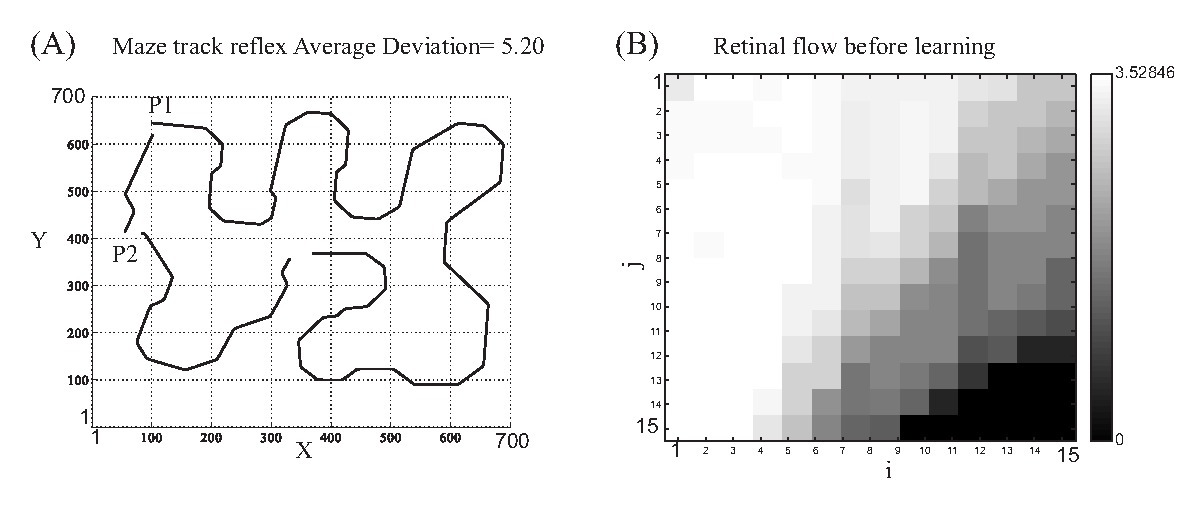
\includegraphics[width=0.9\textwidth]{figures/ppmeasure/8}
	\end{center}
	\caption[Reflex only robot on the maze track]{
	{\bf A)} Trajectory of the robot in the maze track when only the reflex is used ($\mu=0$). 
	{\bf B)} Mutual information $MI(Z,E_{1,i,j})_{t=0}$ for the retina computed during a track run
        \label{PPmeasure:MazeFinalReflex}}
\end{figure}

\begin{figure}[!hbt]
	\begin{center}
		\includegraphics[width=0.9\textwidth]{figures/ppmeasure/9}
	\end{center}
	\caption[Full learning robot on the maze track]{
	{\bf A)} Trajectory of the robot in the maze track during a full learning session.
	{\bf B)} The average retinal field plotted against time. The learning is stable in Stage 1 and Stage 2.
There are 2 phases during the run marked with $[P1,P2]$ and $[P3,P4]$ where the robot does not learn
anything new.
	{\bf C)} Retinal field is constant during Stage 1.
	{\bf D)} Predictive performance in Stage 1. 
	{\bf E)} Retinal field is constant during Stage 2.
	{\bf F)} Predictive performance in Stage 2. 
	\label{PPmeasure:MazeFinalLearning}
	}
\end{figure}

\subsection{Results: application of PP to social systems \label{Chapter8:PPsocial}}

The predictive performance can be applied then to the social system
setting described in Section \ref{Chapter6:Information Flow} where
I already computed the required values.
Figure \ref{fig:PPmeasure:social}, left column shows the outcome of computing the predictive
performance measure for the food and others attraction behaviour.
The white bars contain the PP measure for the attraction behaviour $PP_{Fo}$, whereas
the black bars contain the PP measure for the others attraction behaviour $PP_{Af}$.
I have applied the measure for 3 different scenarios:
\begin{itemize}
 \item a group of $N=10$ agents and $M=5$ food sources, generates five seekers and five parasites.
The agents identified with $1,7,3,9,2$ have $PP_{Fo}> PP_{Af}$ therefore they are
seekers.
The agents identified with $5,8,4,10,6$ have $PP_{Fo}< PP_{Af}$ therefore they are
parasites.
 \item a group of $N=10$ agents and $M=2$ food sources, generates two seekers and eight parasites.
The agents identified with $6,5$ have $PP_{Fo}> PP_{Af}$ therefore they are
seekers.
The agents identified with $3,9,2,7,8,4,10,1$ have $PP_{Fo}< PP_{Af}$ therefore they are
parasites.
 \item a group of $N=10$ agents and $M=8$ food sources, generates eight seekers and two parasites.
The agents identified with $5,9$ have $PP_{Fo}> PP_{Af}$ therefore they are
seekers.
The agents identified with $4,10,3,1,2,7,8,6$ have $PP_{Fo}< PP_{Af}$ therefore they are
parasites.
\end{itemize}

This outcome is compared with the weight development as shown in Fig.\ref{fig:PPmeasure:social},
right column where the weight level for each agent is shown.
There is a critical observation between the discrepancy of weight levels and predictive performance:
high weights does not necessary mean high performance.
For each case one can notice that:
\begin{itemize}
 \item a group of $N=10$ agents and $M=5$ food sources (see Fig. \ref{fig:PPmeasure:social:1}): agents numbered 7 and 3 have
an equal performance as agents 9,2 $PP_{7,3}(Af)\simeq PP_{9,2}(Af)$ although their weights are
lower $W_{7,3}(Af) < W_{9,2}(Af)$.
 \item a group of $N=10$ agents and $M=2$ food sources (see Fig. \ref{fig:PPmeasure:social:2}): agents numbered 6 and 5 have
a different performance $PP_{5}(Af) > PP_{6}(Af)$ although their weights are
similar $W_{5}(Af) \simeq W_{5}(Af)$. Agent $2$ has $W_{2}(Fo) \gg W_{2}(Af)$ but
its predictive performance is similar  $PP_{2}(Af) \simeq PP_{2}(Fo)$
 \item a group of $N=10$ agents and $M=8$ food sources (see Fig. \ref{fig:PPmeasure:social:3}): agents numbered 5 and 9 have
an equal performance $PP_{5,9}(Af) \simeq PP_{5,9}(Fo)$ although their weights are
differently distributed $W_{9}(Fo) \gg W_{9}(Af)$.
\end{itemize}

Again like the previous retinal field case, the weights are not a reliable measure of
the performance of the agents.
Especially in a highly dynamical social system, agents can be lucky and just find
food by chance.
One could be tempted to correlate the $PP(Fo),PP(Af)$ with the number of 
successful food bites or food stolen from other agents but this has the same limits
of looking at the weight.
A corresponding verification via an objective measure like $\psi$ in Eq. \ref{deviation}
would require a complex trajectory analysis for each agent in relationship to each others'
trajectories and therefore was not attempted for computational issues and lack of time.
However basing my assumptions on the previous track follower, I am confident that
the predictive measure can be trust and so agents $5,1$ are the best performing
agents in Fig. \ref{fig:PPmeasure:social:2}. 

\begin{figure}[htbp]
    \begin{center}
%
        \subfigure[When there are 10 agents and 5 food sources, 5 seekers and 5 parasites are generated]{%
            \label{fig:PPmeasure:social:1}
            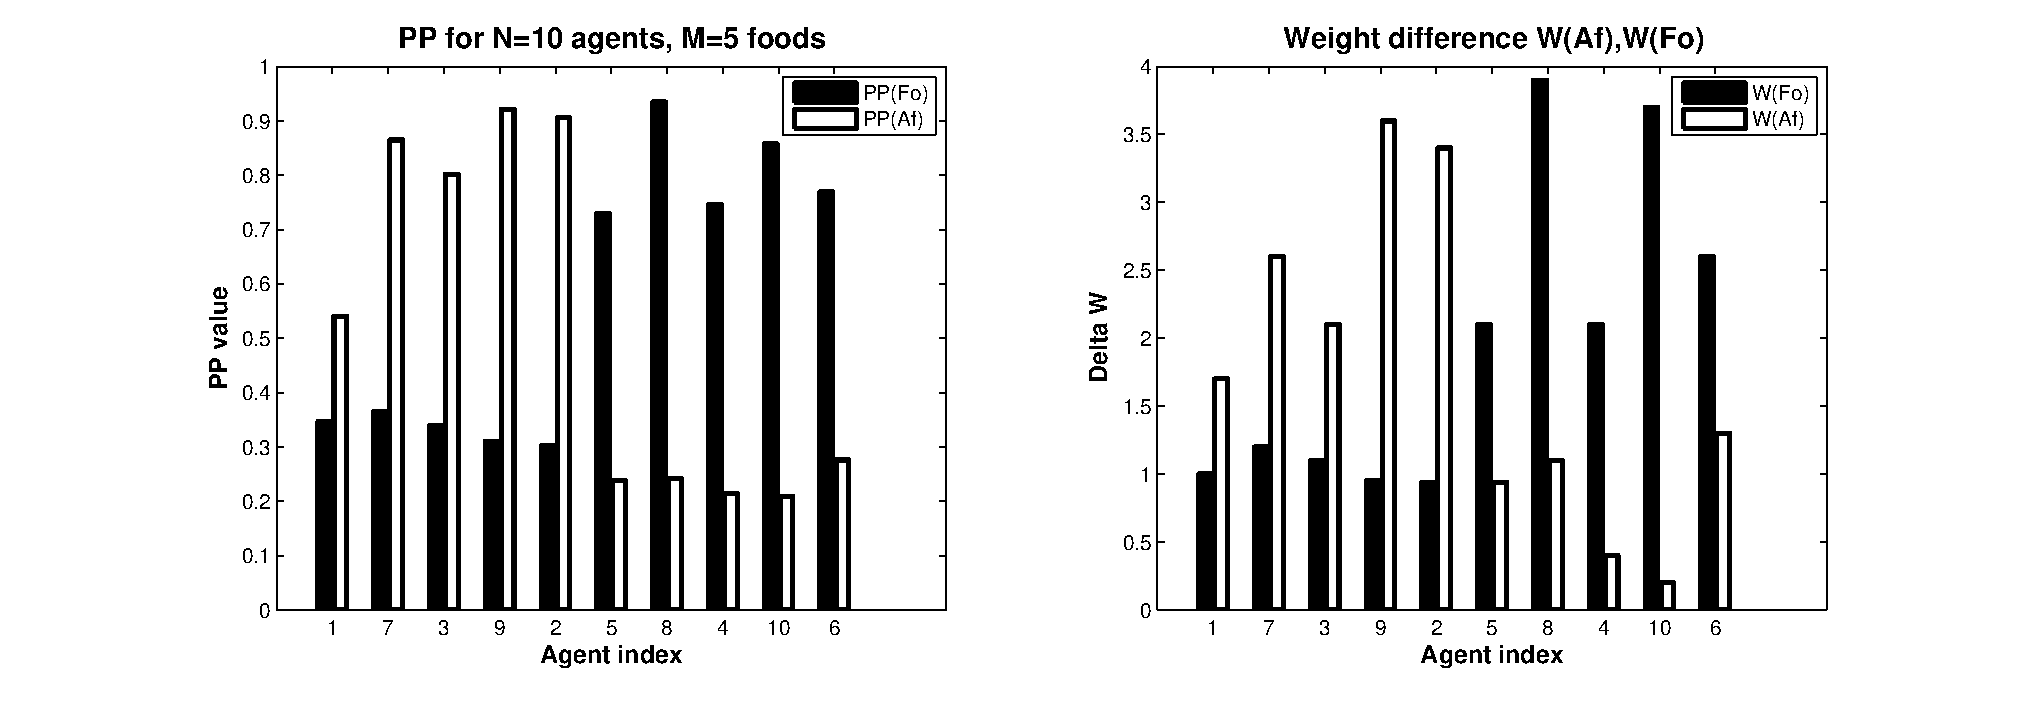
\includegraphics[width=0.9\textwidth]{ppmeasure/social/row1.eps}
        }\\%
        \subfigure[When there are 10 agents and 2 food sources, 2 seekers and 8 parasites are generated]{%
           \label{fig:PPmeasure:social:2}
           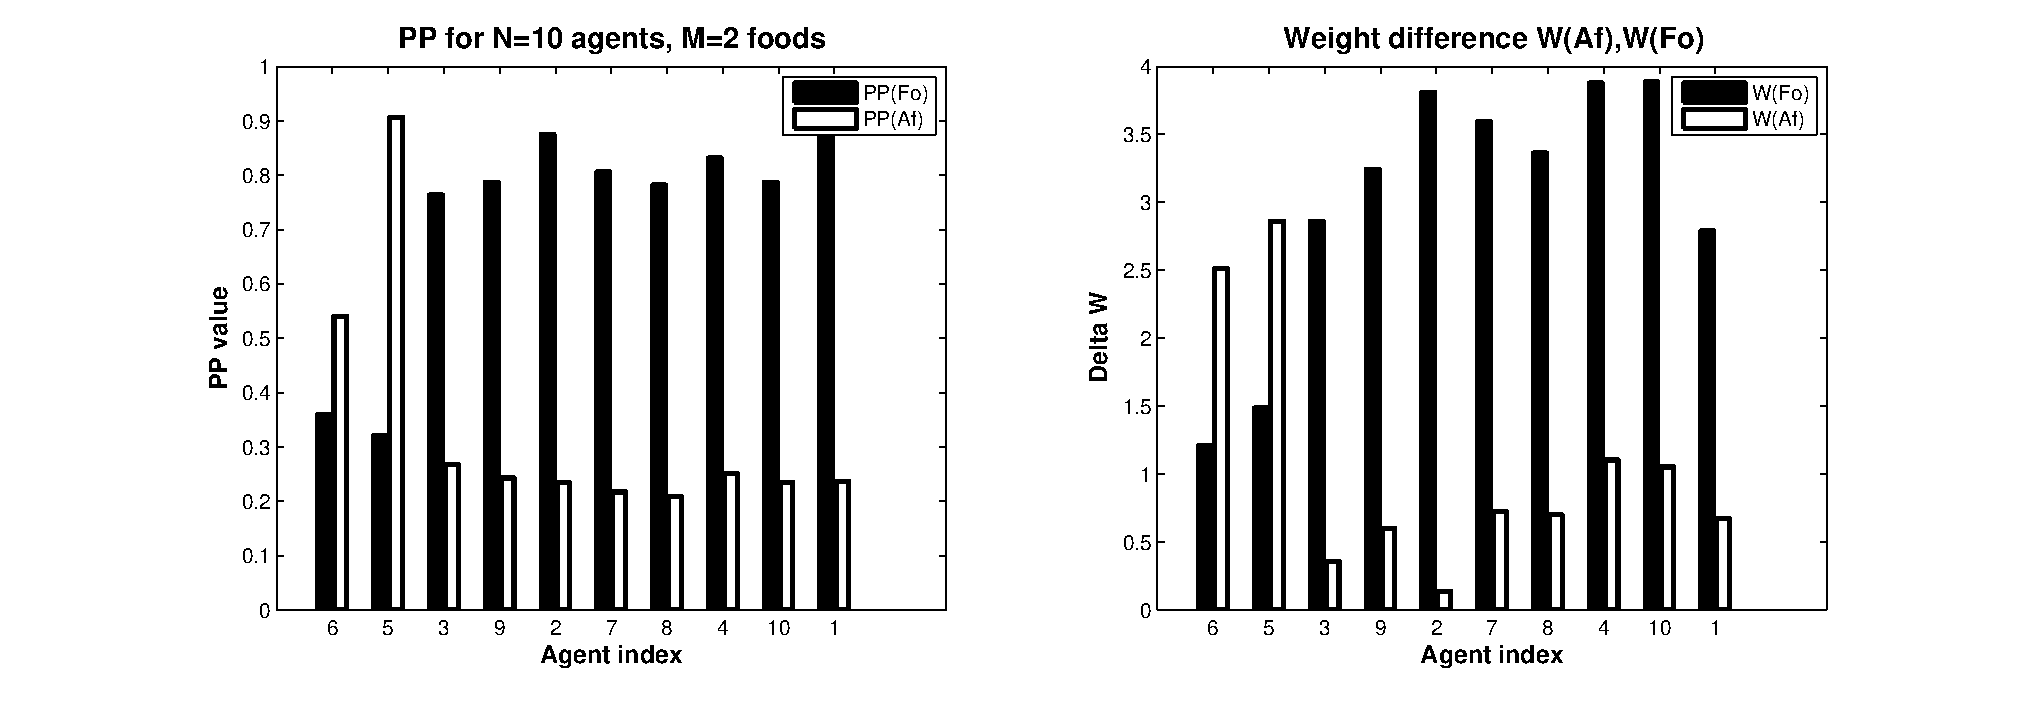
\includegraphics[width=0.9\textwidth]{ppmeasure/social/row2.eps}
        }\\ %  ------- End of the first row ----------------------%
        \subfigure[When there are 10 agents and 8 food sources, 8 seekers and 2 parasites are generated]{%
            \label{fig:PPmeasure:social:3}
            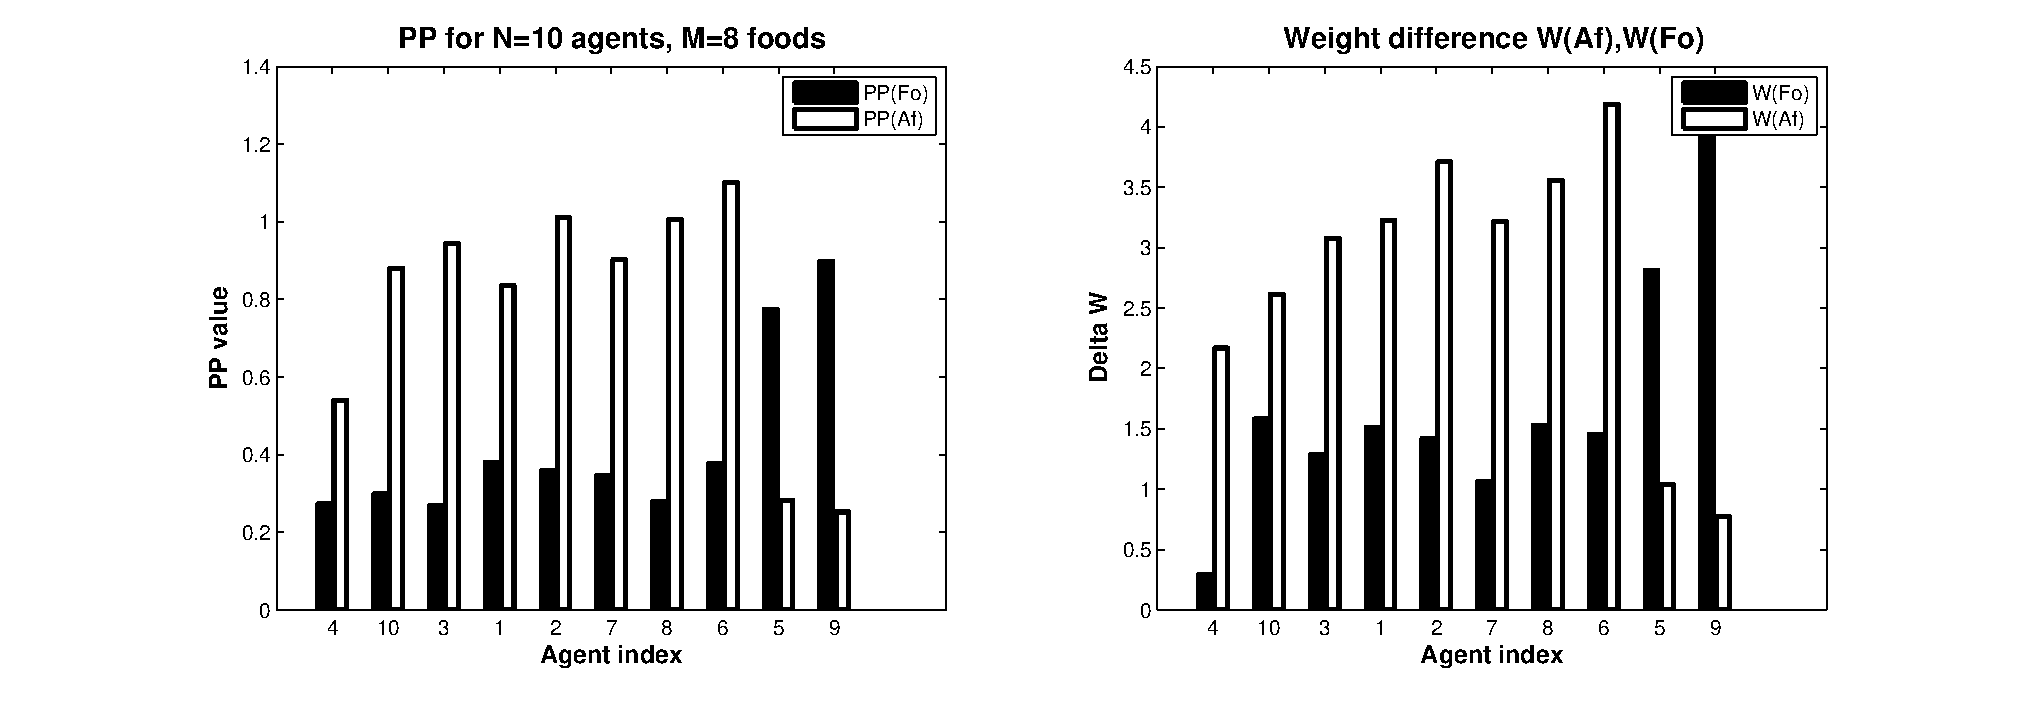
\includegraphics[width=0.9\textwidth]{ppmeasure/social/row3.eps}
        }%
    \end{center}
    \caption[Predictive Measure computed for the social system]{%
     Predictive Measure (PP) computed in the social system for: 
      \textbf{(A)} 10 agents and 5 food sources,
      \textbf{(B)} 10 agents and 2 food sources,
      \textbf{(C)} 10 agents and 8 food sources.
      Left column contains the PP measures with white bars for the food attraction behaviour $PP(Fo)$,
      black bars for the other's attraction behaviour $PP(Af)$.
      Right column contains the weight developed after the system is stabilised for the
      same behaviours $W(Fo),W(Af)$.    \label{fig:PPmeasure:social}
    }
\end{figure}

According to this new results, I can state that the weight are an actual
representation of the social division.
However in the future if the developer wants to use more complex agents
in artificial societies, it will be necessary to compute the $PP$ for 
each behaviour and then compare the different behaviours rather then relying exclusively 
on the weight development.


\subsection{Discussion}

The original Shannon's Information Theory \citep{Shannon76} has been applied
to closed loop systems in several studies like \citet{Ashby1956:IntroCybernetics,Tishby1999:InfoBottle,TouchetteLloyd2004}.
The scope of my predictive performance measure is to unify the Ashby's original theory of requisite variety \citet{Ashby1956:IntroCybernetics}
with the recent frameworks based on mutual information \citep{Tishby1999:InfoBottle} and Bayesian models of perception-action loop \citet{Klyubin2004:Organization,Klyubin2005:Empowerment,Klyubin2007:Representation,Klyubin2008:KeepOptions}.
The Information Bottleneck \citep{Tishby1999:InfoBottle} is an information theoretic framework that finds concise
representations for an `input' random variable that are as relevant as possible for an `output' random variable.
This framework has been used successfully in various supervised and unsupervised applications but cannot be used
as a measure of performance in closed loop controllers.
Building on this initial theoretical work, additional studies were done on
closed loop-systems from an agent-perspective considering the information
 processing properties of such system in the context of what would be
 beneficial for the agent itself \citep{Klyubin2007:Representation,Klyubin2008:KeepOptions,Prokopenko2006:EvolveCoordination,
LungarellaInformationStructure,LungarellaSporns2006:MappingFlow}.
An interesting agent-centric measure called ``empowerment'' was introduced by \citet{Klyubin2005:Empowerment,Klyubin2008:KeepOptions}.
Empowerment is defined as the maximum amount of information that an agent could
send from its actuators to its sensors via the environment, reducing in the simplest
case to the external information channel capacity of the channel from the actuators
to the sensors of the agent.
The empowerment is then used as an utility function that can be maximised
 by the agent's behaviour or by genetic evolution to produce meaningful states.
The empowerment can also be measured  to assess the performance of a general
adaptive agent but it is necessary to disregard the actual behaviour of the agent
and to model how the agent could behave in principle (disregarding the actual
behaviour of the agent can be imagined as removing the agent's controller and
studying the remaining “empty shell” which is the agent's body).

The fundamental difference between the Predictive Performance and empowerment is that
the first is used to quantify the performance of a general adaptive controller
whereas the second is used to drive the controller and at the same time to measure optimality.

Some other studies are focusing specifically on adaptive closed loop systems \citep{Porr2006cf,Kulvicius2010:infomeasure,LungarellaSporns2006:MappingFlow}.
\citet{LungarellaInformationStructure} has proven that for a saliency based attentional behaviour
-based on a PT camera- 
the spatial mutual information increases and entropy decreases around the foveation point.
The information measure was only computed for the visual input of the 
PT camera whereas my predictive performance measure takes into
account the interplay of the sensory motor loop for the driving robot.
Another essential difference with this study is the use
of a purely reflex behaviour whereas my approach includes both
reflex and learning behaviour.

A similar approach was used by \citet{Der2008:PredictiveInfo,Ay2008:PredInformation}
 where the authors defined a predictive information measure $PI$ as the mutual
 information between past and future sensor values to estimate the adaptation
 of a mobile robot to its environment. The mobile robot used in their study was a purely 
reflexive controller described by a parameter $c$ which was chosen to simulate
 different behavioural regimes and how the $PI$ was changing.
Again this study is similar to \citet{LungarellaInformationStructure} because
 is based on a reflex controller and considers only the input:
the transfer entropy is computed between the visual input $S$ and the motor outputs
$M$ for different robot implementations with and without learning.
In the experiment, when the robot is using reward-based learning, the 
transfer entropy is able to track the attention from red objects to blue objects
following a change in the reward signal.
This result is consistent with my observations on the visual flow which shows
how the mobile robot has been adapted to different track shapes.
My Predictive Performance goes further than just measuring the 
information flow because is able to identify if the agent is learning
and being a scalar value avoids the complexities associated with multi dimensional analysis.

\citet{Kulvicius2010:infomeasure} makes a very complete study about 
the adaptive properties of driving robots in a square and circular environments.
The mobile robots are using ICO learning but have only
2 spring antennas rather then a retinal input like my experiment.
The author is able to predict the temporal development of the weights by using an analytical 
model which takes into account the predictive and reflex timing of the input events.
The author then measures energy, input/output ratio and output entropy to 
estimate what is the best antenna ratio for a given environment.
Although their modelling approach is correct, to compute the input/output ratio
one must be able to separate the output contribution of the reflex from the
predictor.
This is not possible in a black box scenario whereas the observer is not able
to discriminate the contribution of the reflex and predictor input.
The speed of learning is then computed as the maximum value of the input/output ratio
and together with the path entropy is used to measure the optimality of the robot.
The path entropy is essentially the output motor entropy and thus indicates
the complexity of the trajectories generated.
The main difference with my work is that I summarize the performance 
of the agent to one value which tells us how good the agent is learning.

The development of the predictive performance is motivated by the original 
paper of \citet{Porr2006cf} where the predictive information is
 computed by summing the weights of the ICO learning rule \citep{Porr2003b}:
the higher the weights the higher is the predictive information.
There are 2 issues with this approach:
firstly I trust what the agent has learned without looking at the
 environment's feedback, secondly it can only be applied to ICO/ISO learning agents.
In the simple case of \citet{Porr2006cf} where the robot 
is using only one ICO neuron the predictive information
 is reliable but it cannot be applied to my case where the retinal
 input is multi dimensional.

The development of visual receptive fields, for example in the primary
visual cortex, has been an intriguing problem addressed in numerous
studies
\citep{Olshausen96,Blais98receptivefield,Weber99orientationselective,Hurri03:SimpleCellReceptive,Kording04:HowAreCell,Wyss06:ModelVentralVisual}.
Whereas in these previous studies the agents operate in open-loop, my
agent learns in a closed loop manner as proposed by
\citet{McKinstry06:CerebellarModel}. The development of the receptive field has been
investigated already by \citet{Kulvicius2007:RFrobot,Kulvicius2010:RFinformation}
which shows that RF can drive the motors of the robot in order to
create better and more stable behaviour, and that development will
stop as soon as the system has obtained behavioural stability after
learning.

In summary, in this study I have analysed an adaptive predictive controller
with the intention to quantify the information used effectively by the robot 
before and after learning.
I introduced the predictive performance to measure the learning ability
of the robot in different tracks.
The robot is facing tracks with increasing difficulty -increasing curvature ratio- 
and is always learning to follow the tracks.
I demonstrated that the predictive performance computed from the agent's 
perspective is consistent with the objective performance on the track.
Additionally I argue that there is a limit in the potential information that an agent can learn,
that enable us to set an upper bound for normalisation purposes.
So the predictive performance help us to measure how much information flow 
the robot is using to achieve its goal without being biased by the absolute weight development.
The predictive performance can be applied to every type of predictive adaptive control 
as long as the predictive and reflex inputs can be identified and is a useful tool 
that can can be used to give an objective estimate of the performance by evaluating information at the subjective level.
The predictive performance is also very useful to determine the performance in the
social system scenario where the highly dynamical setup does not allow the estimation
of an agent performance by looking at the weights.



